% document formatting
\documentclass[10pt]{article}
\usepackage[utf8]{inputenc}
\usepackage[left=1in,right=1in,top=1in,bottom=1in]{geometry}
\usepackage[T1]{fontenc}
\usepackage{xcolor}

% math symbols, etc.
\usepackage{amsmath, amsfonts, amssymb, amsthm}

% lists
\usepackage{enumerate}

% images
\usepackage{graphicx} % for images
\usepackage{tikz}

% code blocks
% \usepackage{minted, listings} 

% verbatim greek
\usepackage{alphabeta}

\graphicspath{{./assets/images/Week 3}}

\title{02-613 Week 3 \\ \large{Algorithms and Advanced Data Structures}}
 
\author{Aidan Jan}

\date{\today}

\begin{document}
\maketitle

\section*{Graph Traversal Algorithms}
\subsection*{Depth First Search (DFS)}
\begin{itemize}
	\item Start from the root node and go down as deep as possible into a branch, and record nodes along the way.
	\item If there are no more child nodes, backtrack the path taken, and go down a different branch.
	\item Since each node in the graph is visited exactly once, this is a O($n$) operation.
	\item Typically implemented using recursion or a stack.
\end{itemize}

\subsubsection*{Theorem}
If $(x, y) \in E$, either $x$ is an \underline{ancestor} of $y$ or $x$ is a \underline{descendant} of $y$.  Proof:
\begin{itemize}
	\item Without loss of generality, $x$ is an ancestor of $y$. 
	\item All nodes between initially seeing $x$ or leaving $x$ are descendents of $x$.
	\item $y$ must be explored before leaving $x$
\end{itemize}

\subsection*{Breadth First Search (BFS)}
\begin{itemize}
	\item Very similar to DFS but rather than going down all one branch all the way, it visits every child in order of level.
	\item Start from the root and record it plus every child.  Repeat for each child in order.
	\item Also O($n$), since each node in the graph is visited exactly once.
	\item Typically implemented using a queue.
\end{itemize}

\subsubsection*{Theorem}
If $(x, y) \in E$, then $|\text{layer}(x) - \text{layer}(y)| \leq 1$. Proof:
\begin{itemize}
	\item Without loss of generality, assume that layer($x$) < layer($y$) - 1.  
	\item All neighbors of $x$ are added in or before layer$(x) + 1$
	\begin{align*}
        \text{layer}(y) &\leq \text{layer}(x) + 1 \\
        \text{layer}(y) &> \text{layer}(x) + 1
    \end{align*}
    \item The above is a contradiction.
    \item Basically, every time a node is visited, all its neighbors are added to the list to be iterated in the next level iteration.
\end{itemize}

The following is an example implementation of BFS.
\begin{verbatim}
TreeGrowing(graph G, node V, function findNext):
    T = ({v}, {})
    S = set of nodes incident to V
    while S != {}
        e = nextEdge(G, S)
        T += e
        S = updateFrontier(G, S, e)
\end{verbatim}

\subsubsection*{Aside: Stacks and Queues}
A queue is an array that views items in a First-in, First-out (FIFO) order.  Basically elements added into the queue first will also be visited first.
\begin{itemize}
	\item \texttt{Dequeue()}: removes the first element of the queue, and moves the head pointer to the next element.
	\item \texttt{Enqueue(e)}: adds the element $e$ to the end of the list.
\end{itemize}
A stack is an array that views items in a Last-in, First-out (LIFO) order.  Basically elements added into the queue last will be visited first.
\begin{itemize}
	\item \texttt{Pop(e)}: removes the last element of the list and decrements the tail pointer to the previous element.
    \item \texttt{Push(e)}: adds an element $e$ to the end of the list.
\end{itemize}

\section*{Bipartite Graphs}
A \textbf{bibartite graph} is one with nodes in two sets such that there are no edges within a partition.
\begin{center}
    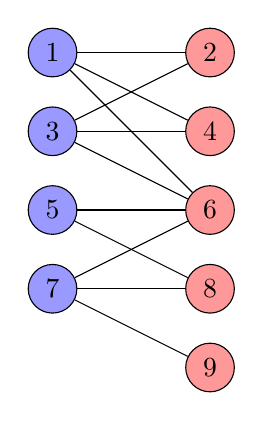
\begin{tikzpicture}
        \node[draw, circle, fill=white!60!blue] at (0, 0) (1) {1};
        \node[draw, circle, fill=white!60!red] at (2, 0) (2) {2};
        \node[draw, circle, fill=white!60!blue] at (0, -1) (3) {3};
        \node[draw, circle, fill=white!60!red] at (2, -1) (4) {4};
        \node[draw, circle, fill=white!60!blue] at (0, -2) (5) {5};
        \node[draw, circle, fill=white!60!red] at (2, -2) (6) {6};
        \node[draw, circle, fill=white!60!blue] at (0, -3) (7) {7};
        \node[draw, circle, fill=white!60!red] at (2, -3) (8) {8};
        \node[draw, circle, fill=white!60!red] at (2, -4) (9) {9};
        \draw (1) edge (2);
        \draw (1) edge (4);
        \draw (1) edge (6);
        \draw (3) edge (2);
        \draw (3) edge (4);
        \draw (3) edge (6);
        \draw (5) edge (6);
        \draw (5) edge (8);
        \draw (7) edge (6);
        \draw (7) edge (8);
        \draw (7) edge (9);
    \end{tikzpicture}
\end{center}
\begin{itemize}
    \item $G = (U\cup V, E)$ such that $U \cap V = \emptyset$
    \item For a graph to be bipartite, it must have a two-coloring.
    \item It must also have no odd-length cycles.
\end{itemize}
Another example:
\begin{center}
    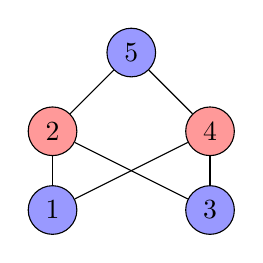
\begin{tikzpicture}
            \node[draw, circle, fill=white!60!blue] at (0, 0) (1) {1};
            \node[draw, circle, fill=white!60!red] at (0, 1) (2) {2};
            \node[draw, circle, fill=white!60!blue] at (2, 0) (3) {3};
            \node[draw, circle, fill=white!60!red] at (2, 1) (4) {4};
            \node[draw, circle, fill=white!60!blue] at (1, 2) (5) {5};
            \draw (1) edge (2);
            \draw (1) edge (4);
            \draw (3) edge (2);
            \draw (3) edge (4);
            \draw (2) edge (5);
            \draw (4) edge (5);
    \end{tikzpicture}
\end{center}
It is easy to tell that this graph is bipartite just by looking at it and coloring it in.  However, what if the graph was bigger?

\subsection*{Breadth-First-Search Strategy}
\begin{enumerate}
	\item First, pick a random node, and BFS through the graph.  Notice that every tree is bipartite since there are no cycles.
	\item Now, insert in all the non-tree-edges.  If there are no edges within the same level, then it is bipartite.  (No "monolayer" edegs.)
\end{enumerate}
\begin{verbatim}
def determineIfBipartite(G):
    T = BFS(G)
    for each layer:
        for each node pair u, v in layer:
            if (u, v) in G.E:
                return False
    return True
\end{verbatim}
\subsubsection*{Proof of Correctness}
For the purpose of contradiction, assume that there exists a $(u, v) \in E$ that is monolayer.  Let $Z$ be the common ancestor of $u$ and $v$ and let the path length from $Z$ to $u$ and $v$ be $l_i$.  In this case, edge $(u, v)$ will create a cycle with length $2 l_i + 1$.  This length is always odd for any $l_i \in \mathbb{Z}$, and results in a contradiction since bipartite graphs cannot have odd-length cycles.  This algorithm will have a time complexity of O($|V| + |E|$) since it is limited by the BFS step.

\section*{Topological Sort}
Given a DAG (directed, acyclic graph), find a bijective mapping $f$ from $v$ to $\{1, \dots, |V|\}$ such that $\forall (u, v) f(u) < f(v)$.


\end{document}